% $Author: ruben $
% $Date: 2010-05-09 22:31:50 $
% $Revision: 1.2 $

% For the FujabaDays 2006
\documentclass[submission,copyright,creativecommons]{eptcs}
\providecommand{\event}{TTC 2016} % Name of the event you are submitting to


\usepackage{graphicx,float,enumerate}
\usepackage{listings}
\usepackage{color}
\usepackage{wrapfig}

\graphicspath{{images/}}

\newcommand{\code}{\texttt}
\newcommand{\p}[1]{\textsf{#1}}


\setlength{\textwidth}{16.5cm}
\setlength{\oddsidemargin}{0cm}
\setlength{\evensidemargin}{0cm}
\setlength{\topmargin}{0cm}

\begin{document}

\definecolor{lightgray}{rgb}{.9,.9,.9}
\definecolor{darkgray}{rgb}{.4,.4,.4}
\definecolor{purple}{rgb}{0.5, 0, 0.33}
\definecolor{commentgreen}{rgb}{0.25,0.5,0.37} 
\definecolor{stringblue}{rgb}{0.16, 0, 1}
\definecolor{annotationgrey}{rgb}{0.39,0.39,0.39}


\lstdefinelanguage{Java}{
  keywords={typeof, try, long, void, new, true, false, catch, function, return,
  null, catch, switch, var, if, in, while, do, else, case, break, private, 
  protected,
  final, static, public, class, implements, extends, boolean, throws, throw,
  this, int, float, double}, 
  keywordstyle=\color{purple}\bfseries, ndkeywords={export}, 
  ndkeywordstyle=\color{darkgray}\bfseries,
  identifierstyle=\color{black},
  sensitive=true,
  comment=[l]{//},
  morecomment=[s]{/*}{*/},
  commentstyle=\color{commentgreen}\ttfamily,
  stringstyle=\color{stringblue}\ttfamily,
  morestring=[b]',
  morestring=[b]", 
  moredelim=[il][\textcolor{annotationgrey}]{$$},
  moredelim=[is][\textcolor{annotationgrey}]{\%\%}{\%\%}
}



\pagestyle{headings}

\title{The SDMLib solution to the Class Responsibility Assignment Case for TTC2016} 
\author{Christoph Eickhoff, Lennert Raesch, Albert Z{\"u}ndorf
\institute{
Kassel University, Software Engineering Research Group,\\
Wilhelmsh{\"o}her Allee 73, 34121 Kassel, Germany\\
\email{raesch|christoph|zuendorf@uni-kassel.de}
}}

\def\authorrunning{ Albert Z{\"u}ndorf}
\def\titlerunning{The SDMLib solution for TTC2016}

\maketitle

\begin{abstract}

This paper describes the SDMLib solution to the Class Responsibility Assignment Case 
for TTC2016. SDMLib provides reachability graph computation ala Groove. Thus, 
the simple idea was to provide rules for possible clustering operations and then use the
reachability graph computation to generate all possible clusterings. Then, we apply the
CRAIndex computation to each generated clustering and identify the best clustering. Of course,
this runs into scalability problems, very soon. Thus, we extended our reachability graph 
computation to do an A* based search space exploration. Therefore, we passed the CRAIndex 
computation as a metric to our reachability graph computation and in each step, we consider 
the set of not yet expanded graphs and choose the one, that has the best metric value for 
expansion. The paper reports about the results we achieved with this approach.  
   
  
\end{abstract}

\section{Introduction}
\label{sec:intro}

This paper describes the SDMLib solution to the Class Responsibility Assignment Case for TTC2016
\cite{ttc2016-case}. SDMLib provides \emph{reachability graph computation} ala Groove 
\cite{rensink2003groove}. For a given start graph and a given set of rules, 
the reachability graph computation generates all graphs that may be derived from 
the start graph by applying all rules at all 
possible matches as often as possible in all possible orders. Each time a new 
graph is 
computed, we search through the set of already computed graphs for an already known 
isomorphic graph. As proposed by \cite{rensink2003groove}, SDMLib computes node and graph 
certificates which are then used as hash keys to access potentially isomorphic 
graphs efficiently. The node certificates then also help to do the actual 
isomorphism test. If a new 
graph has been generated, we create a so-called \emph{reachable state 
node} and we connect the reachable state node of the predecessor graph with the reachable 
state node for the new graph via a rule application edge labeled with the name of 
the rule used. In addition, a root node of the graph is attached to the reachable state node. 
Altogether, the generated reachability graph has a top layer consisting of reachable 
state nodes connected via rule application edges and each reachable state node refers to 
the corresponding application graph via a \texttt{graphRoot} link. In SDMLib, this whole 
structure is again a graph, and graph rules may be applied to it in order to find e.g. 
reachable states with a maximal metric value for the attached application graph 
or to find states 
where all successor states have lower metric values or to find the shortest path leading to 
the best state. Actually, any graph related algorithm may be deployed.  

The Class Responsibility Assignment Case challenges the rule orchestration mechanisms 
provided by the different model transformation approaches. Thus, our solution uses the SDMLib 
reachability graph computation for rule orchestration. This is a very simple way to apply 
all rules in all possible ways and in addition we are able to investigate all intermediate 
results in order to identify which paths through the search space are the most interesting 
ones. The drawback of this approach is that it wastes a lot of runtime and memory space 
for copying the whole class model graph each time a rule is applied and for the search of 
already known isomorphic copies of the generated graphs. As shown in the case 
description, the number of possible clusterings grows with the Bell number, i.e. 
for larger examples a complete enumeration of all possible clustering is not possible in a 
meaningful time. As only a small fraction of the search space can be explored, it might be 
helpful to be able to investigate all intermediate states to identify the most promising spots 
for further expansion. Thus, we hope that the flexibility provided by the SDMLib reachability 
graphs to investigate different intermediate states pays off, in the end. 

As it is usually not possible to generate the whole reachability graph for a given example, 
our reachability graph computation may be restricted to a maximum number of reachable 
states to be generated. Next, we have extended our reachability graph computation with an A* 
like search space exploration that takes a metric as parameter and at each step chooses the 
state with the best metric value for expansion. We have developed two variants of this A* 
algorithm which will be discussed below. 

The next section introduces the rules we use to solve the Class Responsibility Assignment Case
and then Section~\ref{sec:expansion} shows the different search strategies we use in this 
example. Finally, Section~\ref{sec:results} shows our performance measurements. 
 

\section{The Model Transformation Rules}
\label{sec:rules}

Our feature clustering approach uses two SDMLib model transformation rules. In the 
preparation phase we use the rule shown in Figure~\ref{fig:RuleInitialClasses} to create 
one class for each feature in our class model. 

\begin{figure}[ht] \centering
	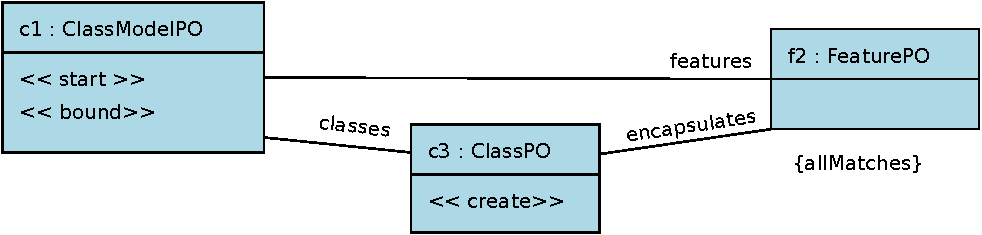
\includegraphics[width=\linewidth]{images/RuleAddInitialClasses.pdf}
 \caption{Rule adding initial classes}
 \label{fig:RuleInitialClasses}
\end{figure}

This rule starts by matching the pattern object \texttt{c1} to the 
\texttt{ClassModel} object passed as parameter. Then, \texttt{f2} is matched to a 
Feature object attached to this \texttt{ClassModel} object. The 
\texttt{\{allMatches\}} constraint causes the rule to be applied to all possible 
matches. Thus, for each \texttt{Feature} object in our current 
\texttt{ClassModel}, the \texttt {$<<$create$>>$ } sterotype on pattern object 
\texttt{c3} causes the creation of a new \texttt{Class} object. In addition 
the new \texttt{Class} object is attached to the \texttt{ClassModel} via a 
\texttt{classes} link and to the \texttt{Feature} object via an 
\texttt{encapsulates} link. Finally, the new \texttt{Class} object's \texttt{name} 
attribute gets assigned the concatenation of the prefix \texttt{"Class4"} 
and the \texttt{name} of the current \texttt{Feature}. Thus, after the 
execution of this rule, each feature has its own class containing just this 
feature. This class model is then used as starting point for the repetitive 
application of our clustering rule. 

 
\begin{figure}[ht] \centering
	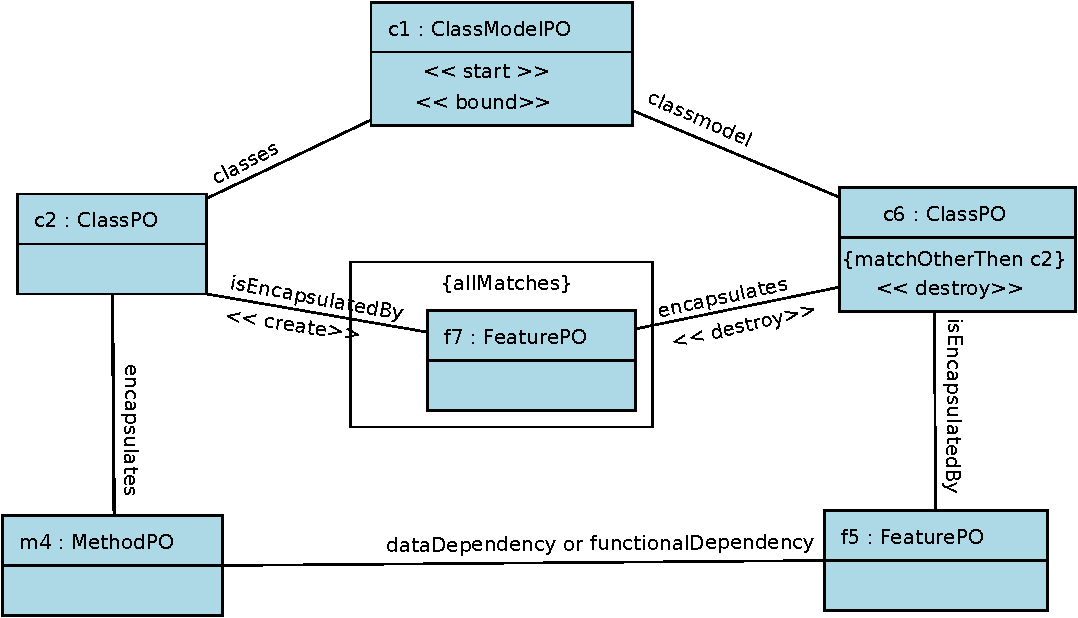
\includegraphics[width=\linewidth]{images/RuleMergeDep.pdf}
 \caption{Merging Classes via Feature Dependencies}
 \label{fig:MergeAttributeRule}
\end{figure}  

Our clustering rule merges classes along functional or data dependencies, 
cf. Figure~\ref{fig:MergeAttributeRule}. The matching of this rule starts with the \texttt{ClassModel} object which 
is bound to \texttt{c1} at rule invocation. Then we follow a \texttt{classes}
 edge to find a match for \texttt{c2}, i.e. a \texttt{Class} object in our 
\texttt{ClassModel}. Next, we follow an \texttt{encapsulates} edge to match 
a \texttt{Method} object \texttt{m4} contained in \texttt{c2}. The object 
matched by \texttt{m4} must have a \texttt{dataDependency} edge 
or a \texttt{functionalDependency} edge to a \texttt{Feature} object 
matched by the pattern object \texttt{f5}. This 
\texttt{Feature} object in turn must be contained in a \texttt{Class} matched by 
\texttt{c6}. By default, SDMLib allows homomorphic matches, thus \texttt{c2} 
and \texttt{c6} would be allowed to match the same \texttt{Class} object. 
Via the \texttt{\{matchOtherThen c2\}} clause, we enforce isomorphic 
matching, i.e. \texttt{c2} and \texttt{c6} must match two different 
\texttt{Class} objects. Finally, the Class matched by \texttt{c6} must belong to our 
\texttt{ClassModel} \texttt{c1}. When such a match is found, the subpattern 
containing the \texttt{FeaturePO} pattern object \texttt{f7} is executed on 
all possible matches. Pattern object \texttt{f7} matches for all features 
contained in the \texttt{Class} matched by \texttt{c6}. (Note, \texttt{f7} 
exploits homomorphic matching and will also match the \texttt{Feature} 
object already matched by \texttt{f5}.) For each \texttt{Feature} object, 
the \texttt{encapsulates} edge connecting it to the \texttt{Class} matched 
by \texttt{c6} is deleted and a new \texttt{isEncapsulatedBy} edge 
connecting it to the \texttt{Class} matched by \texttt{c2} is created. After 
transferring all features to the \texttt{Class} matched by \texttt{c2}, the 
\texttt{Class} matched by \texttt{c6} is destroyed. Thus, the rule shown in 
Figure~\ref{fig:MergeAttributeRule} merges two classes that are connected 
via a feature dependency into one class. 

Our clustering rule merges classes only if there is a dependency between them. 
This already utilizes application specific knowledge about our CRAIndex metric. Our 
search space expansion will start with classes containing only one feature each. Merging 
classes without a dependency between them is not going to improve the CRAIndex of 
the resulting class model. Merging classes has the potential to improve the CRAIndex only 
if the classes contain features that depend on each other. Thus, our clustering rule 
is already optimized for the optimization of the CRAIndex. Using a different metric would 
perhaps require a more general clustering strategy. As the metric is evaluated 
during the search space exploration, it would be easy to simply merge any two 
classes, as any graphs resulting from applying a non metric improving rule 
would immediately be dismissed anyways.


\section{The Search Space Exploration Mechanisms}
\label{sec:expansion}

At the beginning, a \texttt{ReachbilityGraph} object is initialized with a 
start graph or \texttt{startState} and with a set of \texttt{rules} that 
shall be applied to the different reachable states. Our standard A* search space 
exploration algorithm is shown in 
Listing~\ref{lst:defaultAStar}. For the A* search space 
exploration, we call e.g.
\begin{verbatim}
rg.explore(25000, g -> CRAIndexCalculator.calculateCRAIndex((ClassModel) g));
\end{verbatim}
where the first parameter is the maximal number of 
states to be generated and the second parameter is the metric function that guides
our search space expansion algorithm. First, our expansion algorithm initializes 
its \texttt{todo} list with the \texttt{startState} and adds the 
\texttt{startState} to a hash table of reachable \texttt{states} where 
a graph \texttt{certificate} is used as key, as proposed by \cite{rensink2003groove}.
Then, line~5 loops through the \texttt{todo} list until it drains or the maximal 
\texttt{depth} of the search space is reached. 
Line~6 of our explore method just \texttt{sort}s the \texttt{todo} list before choosing 
a new element in line~7. Thereby, each exploration step considers the state with the best 
CRAIndex for further expansion resulting in a depth first like expansion strategy. 
Then line~8 and line~9 iterate through all \texttt{rules} and all matches. 
For each match, we \texttt{clone()} the \texttt{current} state and \texttt{apply()} the 
rule changes to that clone, resulting in a \texttt{newState}. As the \texttt{newState}
may have been created by other rule applications already, line~11 tries to \texttt{find} 
an \texttt{isoOldState}, i.e. the \texttt{find}  operation computes the 
\texttt{certificate} of the \texttt{newState} and tries to look it up in the 
\texttt{states} hash table. This involves an isomorphism check to exclude accidentally 
matching certificates. If no \texttt{isoOldState} is found, line~13 adds the 
\texttt{newState} to the hash table of reachable \texttt{states}, line~14 adds an edge
labeled with the applied rule from the \texttt{current} state to the \texttt{newState}, 
and line~15 adds the \texttt{newState} to our \texttt{todo} list. If there is an 
\texttt{isoOldState} line~17 just adds an edge from the \texttt{current} state to the 
\texttt{isoOldState}.


\begin{lstlisting}[language=Java, numbers=left, captionpos=b, 
label={lst:defaultAStar}, escapeinside={\%}{\%},
caption={Default A* based Search Space Expansion}
]
ReachabilityGraph::explore(depth, metric) {
   todo = new ArrayList();
   todo.add(this.startState);
   states.put(certificate(this.startState), startState);
   while (! todo.isEmpty() && states.size() <= depth) {
      sort(todo, metric);
      current = todo.get(0); todo.remove(0);
      for(Rule r : this.rules) {
         while (r.findMatch()) {
            newState = current.clone().apply(r);
            isoOldState = find(states, newState);
            if (isoOldState == null){
               states.put(certificate(newState), newState);
               addEdge(current, r, newState);
               todo.add(newState);
            } else {
               addEdge(current, r, isoOldState);
            }
         }
      }
   }
}
\end{lstlisting}


Within each step, our default A$*$ search space exploration strategy 
generates all successors of the 
\texttt{current} state. For case E there are about 400 dependencies, thus, 
the initial state has about 400 successor states. While this number decreases 
by one with each rule application, the first 100 rule applications  
have 350 successors on average resulting in 35000 states, which already exceeds our 
memory space. To improve this, we added a variant of our algorithm called 
\emph{Ignore Decline} mode.  The Ignore Decline mode improves our 
exploration algorithm by comparing the metric value of the \texttt{newState} with 
the current \texttt{bestMetric}. If the metric of the \texttt{newState} is lower 
then the \texttt{bestMetric} we ignore the \texttt{newState}, i.e. 
we do not add it to our reachability graph nor to our \texttt{todo} list. This 
may exclude some important candidates from later consideration but it reduces the 
number of states to be added to our reachability graph considerably thus reducing 
memory space consumption.   

The second variant of our search space exploration algorithm is called 
\emph{Promote Improvements} mode.  The Promote Improvement mode computes the metric 
for each new state and in case of an improvement compared to the current state, 
we stop the expansion of the current state (putting it back into the todo list). 
Then we jump back to line~6 and start with a new iteration, i.e. we sort the todo list 
(bringing the new best state to the front) and continue the search space exploration 
with this new state.
The Promote Improvement mode reaches  
local optima of the reachability graph very fast. 
Note, when the search is exhausted for some state and we go back to earlier
states, rule application on those earlier states will first produce the same
matches as in earlier runs. These same old matches will be identified by line~11
as \texttt{isoOldState}s and thus ignored. However, this requires the computation 
of a certificate and an isomorphism check. To avoid this effort, our real 
implementation of the Promote Improvement mode stores 
the number of already created successors
for each state and on reconsideration, this number of rule applications is directly 
ignored.  


\section{Performance Results}
\label{sec:results}

Figure~\ref{fig:PerformanceSummary} shows the CRAIndex we achieve for the 
different input models and the time our best algorithm needed to compute this. 

\begin{figure}[H] \centering
	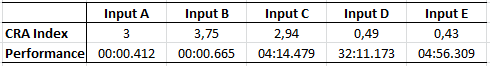
\includegraphics[width=0.8\linewidth]{images/performanceSummary.png}
 \caption{Performance Summary}
 \label{fig:PerformanceSummary}
\end{figure}



\bibliographystyle{abbrv}
\bibliography{fujaba}  

\end{document}

 